\documentclass{article}
\usepackage[utf8]{inputenc}
\usepackage{amsmath} 
\usepackage{graphicx}

\title{Homework 2}
\author{Amol Bhagavathi}
\date{October 11 2024}

\begin{document}
\maketitle

\subsection*{Question 1:}
\textbf{Admissibility and Consistency:} Consider a search space with a single goal state. Prove that if a heuristic is consistent, it must also be admissible.
\subsection*{Answer:}
A heuristic \( h(n) \) is said to be consistent if, for every node \( n \) and every successor \( n' \), it satisfies the inequality:
\[
h(n) \leq c(n, n') + h(n'),
\]
where \( c(n, n') \) is the cost of reaching \( n' \) from \( n \). For the goal state \( G \), we have \( h(G) = 0 \), which implies \( h \) does not overestimate the true cost \( h^*(G) = 0 \).
To show that consistency implies admissibility, assume \( h \) is consistent. We want to prove that \( h(n) \leq h^*(n) \) for all nodes \( n \).
Consider any path from node \( n \) to the goal. The consistency condition ensures that at each step, the heuristic value at node \( n \) is less than or equal to the true cost of reaching the goal from \( n \). Thus, \( h(n) \) cannot overestimate \( h^*(n) \).
Therefore, \( h(n) \leq h^*(n) \) for all \( n \), and \( h \) is admissible.

\subsection*{Question 2:}
\textbf{Search:} Our friend pacman has been dropped into a new 4x4 maze. We notice that there are five food pellets and their position is given to us. Pacman starts at (4,3) as shown in the figure below. As always, Pacman can move UP, DOWN, LEFT, and RIGHT whenever possible. Pacman is very hungry and wants to eat all five food pallets. One of your classmate recalls that she can use search algorithm to help Pacman. So she begins formulating the search problems.
\\
(a) How should she define the start state $S_s$?
\\
(b) We note that the possible actions at our disposal are UP, DOWN, LEFT, and RIGHT. For an action $a \in$ \{UP, DOWN, LEFT, and RIGHT\} at a state $S_n$. How is transition function (or a successor function) $T(S_n, a)$ defined?
\\
(c) Define a goal test $ISGoal(S_n)$?
\\
(d) You want to use A* search to solve the search problem you just defined. Design a heuristic function that is both admissible and consistent?

\subsection*{Answer:}
(a) For each state, she should include the position of Pacman and the number of pellets left to be eaten in a list. Therefore, for the start state $S_s$, we can represent this as $[(4,3), 5]$
\\
(b) Note that $S_n[0]$ gets the position tuple of Pacman. The first value of thh tuple represents the column and the second value represents the row.
\[T(S_n, a) =
\begin{cases}
    S_n[0][0] + 1 & \text{if } a = \text{UP} \\
    S_n[0][0] - 1 & \text{if } a = \text{DOWN} \\
    S_n[0][1] + 1 & \text{if } a = \text{RIGHT} \\
    S_n[0][1] - 1 & \text{if } a = \text{LEFT} \\
    S_n[1] - 1 & \text{if position contains a pellet} \\
\end{cases}
\]
\\
(c) A goal test $S_n$ takes in a state and checks if the second term in the list = 0, i.e if $S_n[1] = 0$, then goal state is reached
\\
(d)

\subsection*{Question 3:}
\textbf{Peaceful Ghost:} Imagine Pacman playing against a peaceful ghost. The ghost
tries to block Pacman from getting to the food pallet. However, the ghost is peaceful in
nature and does not kill pacman. This implies that Pacman and the ghost cannot occupy
the same square. Both Pacman and the ghost can move in any of the four directions.
Neither can remain still. The ghost cannot move into the square with the food pellet.
Pacman's score is the number of pellet it has eaten.
\\
(a) Starting from the position shown above, draw a game tree where each
player moves once for each player. You can assume Pacman moves first.
\\
(b) According to the game tree you draw, what is the value of the game? Use
Pacman's score as your evaluation function.
\\
(c) If we consider 20 moves for each player, what is the value of the game
computed by MiniMax?
\\
(d) Now, imagine we have a more sophisticated layout. For this layout, a
partial game tree is drawn below and the leaf nodes were scored using some evaluation function. Fill in the values of all internal nodes using the MiniMax algorithm. In the same figure, cross off any nodes that are not evaluated when using AlphaBeta pruning. (Assume standard left-to-right tree traversal).
\\
(e) Reorder the leaf nodes such that the number of nodes not visited by Alpha-Beta pruning is maximized, assuming we explore the tree from left to right.
(ii) Now, you are free to re-order children at each level. Redraw the tree with the new ordering such that the maximum level of pruning is achieved.

\subsection*{Answer:}
(a) Note that in the position tuple (x,y), x represents the column and y represents the row
\begin{figure}[h]
    \centering
    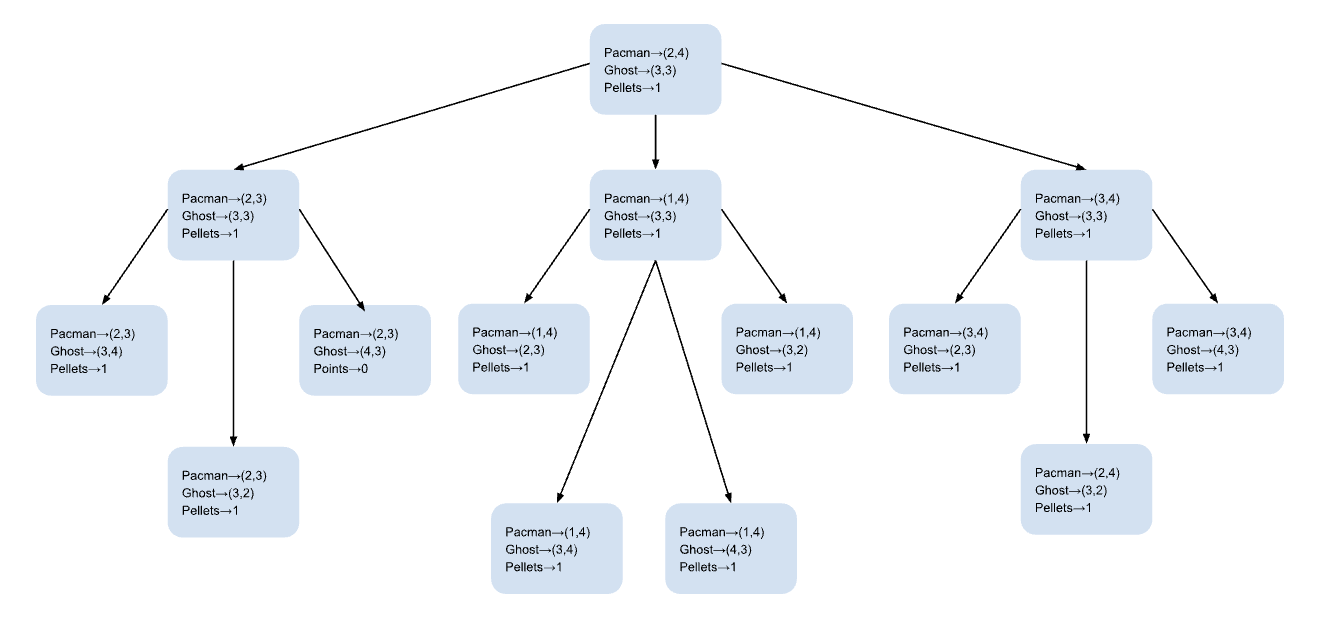
\includegraphics[width=1\textwidth]{part3a.png}
    \caption{Partial Game Tree for 3a}
    \label{fig:sample}
\end{figure}
\\
(b) The value of the game is 0 since Pacman has not eaten any pellets.
\\
(c) The value of the game is 1 since Pacman will always win.
\\
(d) 
\\
(e)


\subsection*{Question 4:}
\textbf{Heuristic Alpha-Beta Tree Search:} Consider the game of tic-tac-toe. We
define $X_n$ as the number of rows, columns, or diagonals with exactly $n $ X's and no O's. Similarly, $O_n$ is the number of rows, columns, or diagonals with just $n$ O's. The utility function assigns +1 to any position with $X_3$ = 1 and -1 to any position with $O_3$ = 1. All other terminal positions have utility 0. For nonterminal positions, we use a linear evaluation function defined as $Eval(s) = 3X_2(s) + X_1(s) - (3O_2(s) + O_1(s))$.
\\
(a) Approximately how many possible games of tic-tac-toe are there?
\\
(b) Show of whole game tree starting from an empty board down to depth 2 (i.e., one X
and one O on the board), \textbf{taking symmetry into account.}
\\
(c) Mark on your tree the evaluations of all the positions at depth 2.
\\
(d) Using the minimax algorithm, mark on your tree the back-up values for the positions at depth 1 and 0, and use those values to choose the best starting move.
\\
(e) Circle and nodes at depth 2 that would \textbf{not} be evaluated if alpha-beta pruning were applied, assuming the nodes are generated in the optimal order for alpha-beta pruning.

\subsection*{Answer:}
(a) Given that each person makes a turn, and there are 9 spaces on board, the number of possible games of tic-tac-toe is $9! = 362,880$
\\
(b) 
\begin{figure}[h]
    \centering
    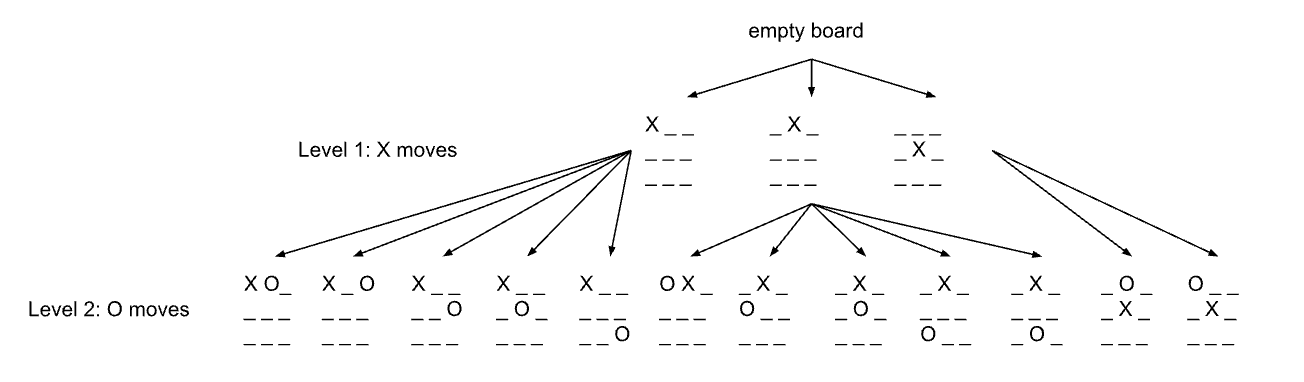
\includegraphics[width=1\textwidth]{part4b.png}
    \caption{Game Tree for 4b}
    \label{fig:sample}
\end{figure}
\\
(c)
\begin{figure}[h]
    \centering
    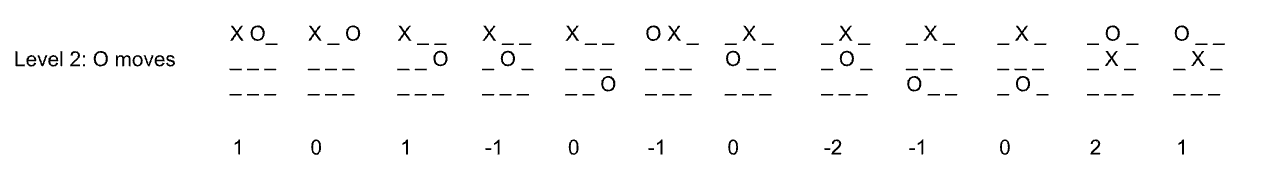
\includegraphics[width=1\textwidth]{part4c.png}
    \caption{Level 2 Evaluations for 4c}
    \label{fig:sample}
\end{figure}
\\
(d)
\begin{figure}[h]
    \centering
    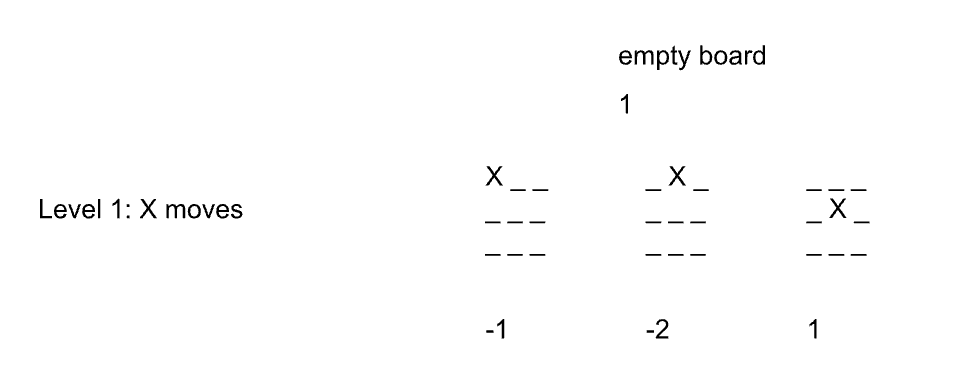
\includegraphics[width=1\textwidth]{part4d.png}
    \caption{Back-up values for 4d}
    \label{fig:sample}
\end{figure}
\\
(e)
\begin{figure}
    \centering
    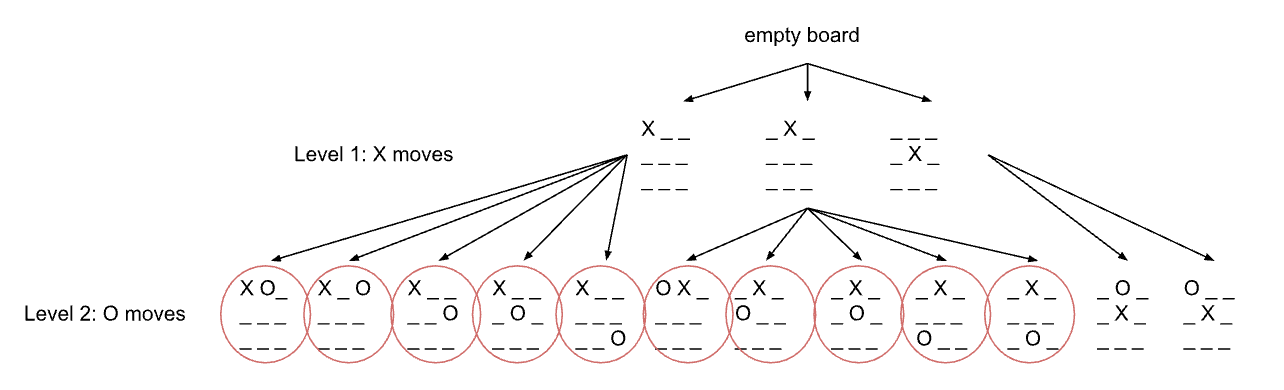
\includegraphics[width=1\textwidth]{part4e.png}
    \caption{Nodes not evaluated for 4e}
    \label{fig:sample}
\end{figure}

\end{document}
